\documentclass[12pt]{article}
\usepackage{cite}
\usepackage[francais]{babel}
\usepackage[utf8]{inputenc}
\usepackage[T1]{fontenc}
\usepackage{url}
\usepackage{graphicx}
\usepackage{lmodern}
\usepackage{amsmath}
\usepackage{amssymb}
\usepackage{mathrsfs}
\usepackage[left=3cm, right=3cm, top=3cm]{geometry}
\begin{document}
\tableofcontents
\newpage
\section{Apprentissage automatique (Machine Learning)}
\subsection{Introduction}
La faculté d'apprendre est essentielle à l'être humain pour reconnaître une voix, une personne, un objet... On distingue en général deux types d'apprentissage: l'apprentissage «par cœur» qui consiste à mémoriser telles quelles des informations, et l'apprentissage par généralisation où l'on apprend à partir d'exemples un modèle qui nous permettra de reconnaître de nouveaux exemples. Pour les systèmes informatiques, il est facile de mémoriser un grand nombre de données (textes, images, vidéos...), mais difficile de généraliser. Par exemple, il leur est difficile de construire un bon modèle d'un objet et d'être ensuite capable de reconnaître efficacement cet objet dans de nouvelles images.

L'apprentissage automatique est une tentative pour comprendre et reproduire cette faculté d'apprentissage dans des systèmes artificiels. Il nous semble donc approprié d'utiliser des techniques issues de ce domaine pour découvrir et modéliser des connaissances liant texte et image.

L'apprentissage automatique se trouve au carrefour de nombreux autres domaines: intelligence artificielle, statistiques, sciences cognitives, théorie des probabilités, de l'optimisation, du signal et de l'information... Il est donc bien difficile de donner une taxonomie des techniques d'apprentissage.

Après avoir donné quelques définitions, nous présentons brièvement dans ce chapitre les deux principaux types d'apprentissage: l'apprentissage supervisé et non-supervisé, et nous donnons pour chacun d'eux quelques exemples de techniques d'apprentissage.
\subsection{Techniques d'apprentissage automatique}
Dans ce mémoire, nous nous intéressons aux techniques d'apprentissage sur de grande masses d'images. Cependant, avant de pouvoir utiliser les techniques d'apprentissage, il est nécessaire de réaliser quelques pré-traitements sur les données. L'ensemble des techniques utilisées avant, pendant et après l'apprentissage sur de grandes masses de données est souvent regroupé sous le terme de Exploration de données dite «Data Mining».

Exploration de données «Data Mining» c’est une technique qui considère tout le processus d'extraction de connaissances à partir d'un grand nombre de données \cite{Grabmeier}. Ses principales étapes sont:
\begin{itemize}
  	  \item L'extraction et le stockage des données.
  	  \item L'exploration des données pour la détection de valeurs aberrantes, atypiques, d'incohérences, et pour la sélection et la transformation des données à étudier...
  	\item Le partitionnement aléatoire des données en trois ensembles: apprentissage, validation et test.
  	\item La réalisation d'un apprentissage numérique ou symbolique à partir des données nettoyées avec estimation de la complexité du modèle et optimisation des paramètres sur l'ensemble de validation.
  	\item La comparaison des résultats obtenus à l'aide des modèles optimaux sur l'ensemble de validation avec les résultats obtenus sur l'ensemble de test afin de tester la capacité de généralisation du modèle.\\
\end{itemize}

Il est utilisé dans de nombreux domaines: bases de données, analyse de données, statistiques, classification, programmation logique, visualisation...
		\subsubsection{Apprentissage}
		La classification supervisée (appelée aussi classement ou classification inductive) à pour objectif d'apprendre par l'exemple. Elle cherche a expliquer et prédire l’appartenance de documents a des classes connues apriori. Ainsi c'est l'ensemble des techniques qui visent a deviner l'appartenance d'un individu a une classe en s'aidant uniquement a des valeurs qu'il prend \cite{Govaert}.

L'apprentissage supervisé suppose qu'un oracle fournit les étiquettes de chaque donnée d'apprentissage l’oracle ici c’est pour chaque xi, fournit une étiquette ui dans U (avec une distribution de probabilité $F(u|x)$ inconnue).

On distingue en général trois types de problèmes auxquels l'apprentissage supervisé est appliqué: la classification supervisée, la régression, et les séries temporelles. Ces trois types de problèmes se différencient en fonction du type d'étiquettes fournit par l'oracle.
Nous présentons maintenant brièvement trois algorithmes classiques d'apprentissage supervisé:
\begin{enumerate}
	\item Les k plus proches voisins (k - NN): déterminer pour chaque nouvel individu que l'on veut classer, la liste des k plus proches voisins parmi les individus déjà classés.
	\item La classification bayésienne: Le classifieur bayésien va choisir la classe Ck qui a la plus grande probabilité, on parle de règle MAP (maximum a posteriori).
	\item Machines à vecteurs de support (SVM): (Support Vector Machines) La méthode à base de SVM cherche l'hyperplan séparateur le plus éloigné des documents du corpus d'apprentissage.
\end{enumerate}

\subsubsection{Apprentissage non-supervisé}
Contrairement à l'apprentissage supervisé, dans l'apprentissage non-supervisé il n'y a pas d'oracle qui explicite les étiquettes. L'utilisation de ce type d'algorithme permet de trouver des structures, des dépendances entre descripteurs... qui nous sont inconnues (on dit aussi latentes). Dans le cadre de ce travail, nous ne nous intéresserons qu'à la régression. Pour ce problème, les étiquettes sont des valeurs.

Le plus connu des problèmes non-supervisés est la classification non-supervisée ou clustering. Les classes, que nous appellerons clusters, sont formées par regroupement des documents qui ont certaines caractéristiques en commun. Un autre problème non-supervisé est l'estimation de densité. Son objectif est de modéliser la distribution des données. Le modèle doit pouvoir fournir une bonne estimation d'un document de test issu de la même distribution (inconnue) que les données d'apprentissage. Son objectif est de résumer l'information importante, de la dissocier du bruit.

Le clustering est un outil important pour l'analyse de données. En français, le mot classification est ambigüe, car il s'agit soit de retrouver la classe à laquelle le document appartient (classification supervisée), soit de construire des regroupements de documents (classification non-supervisée). Pour distinguer ces deux cas, nous parlerons de classement pour la première et de clustering pour la seconde. Le clustering vise à trouver les structures intrinsèques des données en les organisant en groupes homogènes et distincts (les clusters). Les objets dans un même cluster doivent être similaires entre eux et différents des objets des autres clusters [3].\\
Pour construire un regroupement de ces données, un utilisateur a trois choix méthodologiques à faire :
\begin{enumerate}
	\item Choisir une mesure de ressemblance entre les données.
	\item Choisir le type de structure qu'il veut obtenir: partition, hiérarchie, arbre, pyramide.
	\item Choisir la méthode permettant d'obtenir la structure désirée.
\end{enumerate}
On distingue généralement quatre types d'approches du clustering [4]:
\begin{enumerate}
	\item Les approches basées sur le partitionnement des données: les points de données sont diviser en k partition, où chaque partition représente un cluster. La partition est faite sur la base de certains objectif fonction. Une de ces fonctions standard est de minimiser le carrée d’erreur.
	\item Densités: sont définies comme des zones de densité supérieure au reste de l’ensemble de données. Les objets rares dans ces zones - qui sont nécessaires pour séparer les clusters - sont généralement considérés comme du bruit et des points frontières.	
	\item L'espace (grid): utilise une structure de données de grille multi-résolution. Il quantifie l'espace objet en un nombre fini de cellules qui forment une structure de grille sur laquelle toutes les opérations de clustering sont effectuées.
	\item Les approches hiérarchiques: les plus petites cluster sont fusionnées en plus grandes, ou les plus grandes cluster sont découpés en plus petites cluster . Le résultat de l'algorithme est un arbre de cluster, appelé dendrogramme, qui montre la relation entre les cluster.
\end{enumerate}
Nous présentons trois algorithmes classiques d'apprentissage non-supervisé:
\begin{enumerate}
	\item Les k - moyennes (k - means): est un outil de partitionnement des données non-hiérarchique qui permet de répartir les données en k clusters homogènes [5].
	\item Les cartes auto-organisatrices (SOM - self organizing map ou carte de Kohonen (1982)): appartiennent aux techniques de clustering par partitionnement des données. Cette technique est un cas particulier de réseau de neurones non-supervisé [6].
	\item La Classification Ascendante Hiérarchique (CAH): Il appartient à la méthode des heuristiques. Cette méthode est utilisée pour construire des clusters pour les documents ainsi que pour les visualiser [7].
\end{enumerate}
\subsection{Autres types d'apprentissage}
Il existe d'autres types d'apprentissage. Citons l'apprentissage semi-supervisé et l'apprentissage par renforcement. Ces deux types d'apprentissage nous semblent être intéressants pour la recherche d'images.

En effet, l'apprentissage semi-supervisé est un bon compromis entre apprentissage supervisé et non-supervisé, car il permet de traiter un grand nombre de données sans avoir besoin de toutes les étiqueter, et, bien utilisé, il donne de meilleurs résultats que l'apprentissage non-supervisé.

L'apprentissage par renforcement est utile dans le cas d'apprentissage interactif, comme les techniques de bouclage de pertinence.
\subsubsection{Apprentissage semi-supervisé}
L’apprentissage semi-supervisé suppose que l’on dispose de peu de données étiquetées et d’un grand nombre de donnée non étiquetées. L’apprentissage s’effectue alors à partir des deux source de données.
	
Un exemple d'apprentissage semi-supervisé est le co-apprentissage (co-training). L'apprentissage actif est une forme particulière d'apprentissage semi-supervisé, car il consiste à faire annoter par l'utilisateur quelques exemples positifs et négatifs.
	
Il permet d'intervenir dans le processus de construction de l'ensemble d'apprentissage dans le cadre de la recherche interactive. Certaines techniques classiques ont été étendues au cas de l'apprentissage semi-supervisé [8].
\subsubsection{Apprentissage par renforcement}
L’apprentissage par renforcement désigne toute méthode adaptative permettant de résoudre un problème de décision séquentielle. L'apprentissage par renforcement est synonyme d'apprentissage par interaction. Pendant l'apprentissage, le système adaptatif agit en interaction avec son environnement, et en retour reçoit des signaux de renforcement. Son objectif est de maximiser une mesure de gain dépendant des signaux reçus. Le terme adaptatif signifie que l'on part d'une solution inefficace, et qu'elle est améliorée progressivement en fonction de l'expérience du système.
\subsection{Conclusion}
Dans cette partie, nous avons décrit quelques techniques d'apprentissage de différents types (supervisés, non-supervisés, semi-supervisés, par renforcement) qui peuvent être employées pour l'indexation et la recherche d'images.

\newpage
\section{Apprentissage profond (Deep Learning)}
\subsection{Introduction}
Après avoir présenté de manière globale l’apprentissage automatique, nous allons maintenant nous intéresser plus particulièrement à l’apprentissage profond. Pour illustrer la discussion, nous allons d’abord présenter en détail le type de modèle le plus utilisé dans ce contexte: les Réseaux de Neurones Artificiels (ANNs).
\subsection{Apprentissage profond}
La notion d’apprentissage profond est tout d’abord une traduction directe du terme anglais « Deep Learning », que certain préfère traduire par la notion d’apprentissage statistique. De même que sa traduction, sa définition varie également, mais principalement au niveau des détails [10].
Pour définir cette notion dans les grandes lignes, on pourrait dire que L’apprentissage profond est un algorithme d'abstraction de haut niveau qui permet de modéliser les données à partir de grands ensembles de données apprises.\\
Précisons quelques termes [10]:
\begin{itemize}
	\item \textbf{L'abstraction} suppose que les données initiales diffèrent largement des donnés de sorties, avec pour résultat possible la classification d’images, la prédiction d’un comportement ou une traduction. L'abstraction signifie qu'il n'y a pas de relation simple entre l'entrée et la sortie.
	\item \textbf{La modélisation} signifie que nous tentons de créer un certain scenario réaliste de sorte qu'une classification ou un résultat réaliste en découle.
	\item \textbf{La notion relative aux grands ensembles de données} signifie que les données d’entrée sont extrêmement diverses. L'apprentissage profond ou l'apprentissage automatique implique généralement que les propriétés importantes de ces données sont détectées lors du processus d'apprentissage.
\end{itemize}

De nombreux termes de ce utilisés proviennent des sciences neurologiques, notamment de la notion de réseau de neurones. Un réseau neuronal est une sorte de logiciel cérébral ou de machine virtuelle composée de milliers d’unités (les neurones) qui effectuent des calculs. Plus précisément, des unités logiques et de prises de décisions (neurones, perceptrons) relient les données d’entrées et de sorties entre elles par l’intermédiaire d’un réseau complexe (réseau, cerveau) capable de prendre des décisions complexes.

A l'origine, ces systèmes portaient le nom de réseaux artificiels de neurones (ANN, Artificial Neural Networks) afin de les différencier des systèmes biologiques. Ils se composent en général d’un certain nombre de données d'entrées et de sorties (input / output layer), d’un réseau étroit de neurones et de plusieurs strates intermédiaires (hidden layers). Ces couches intermédiaires permettent de traiter des problèmes complexes ; sans elles, le système ne résout que des calculs simples. Le nombre de couches est donc un facteur décisif pour la complexité du système, et de l’apprentissage ; les données s’associent d’une couche à l’autre, les résultats d’une première couche servant d’entrée à la prochaine, et ainsi de suite afin d’aboutir à une prise de décision complexe. Ce fonctionnement en strates donne toute sa profondeur au réseau et à l’apprentissage.
\subsection{Réseaux de Neurones Artificiels (ANNs)}
\subsubsection{Historique}
C’est dans les années 40 que la neurophysiologie a commencé à comprendre le fonctionnement des neurones biologiques, avec notamment les notions d’influx nerveux, de seuil d’activation, d’excitation du neurone et de renforcement de certaines structures par l’apprentissage [11].

Naturellement, les chercheurs essayèrent alors de reproduire un neurone de façon artificielle, d’abord sous forme de circuits électriques puis lorsque les langages de programmation le permirent, sous forme de code. En 1957, “Franck Rosenblatt” invente le “Perceptron”, qui est la première tentative de reconnaissance d’image par un algorithme.

Après un creux dans les années soixante en raison de doutes sur la robustesse théorique de ces modèles, la recherche sur les ANN prit un second souffle en 1986 lorsque l’algorithme dit de « rétro-propagation » (back-propagation) permit de multiplier le nombre de couches d’un ANN et donc sa capacité à reconnaître des concepts de plus en plus complexes. En 1998, “Yann Le Cun” proposa le fameux réseau LeNet-5 pour la reconnaissance de caractères [11].

Mais pénalisés par le manque de données et la puissance limitée des machines de l’époque, les réseaux neuronaux passèrent de mode à nouveau au début des années 2000 au profit d’autres techniques de machine learning. Ce n’est que vers 2010 que débuta l’accélération connue aujourd’hui.
\subsubsection{Le neurone biologique}
L’unité de calcul principal du système nerveux, le neurone, est constitué de trois parties: l’arbre dendritique, le soma et l’axone ; une illustration est présentée à la figure 1. Au repos, l’intérieur du neurone est polarisé négativement par rapport à l’extérieur. Cela est dû à un ensemble de pompes contrôlant les concentrations relatives de différents ions, entre l’intérieur et l’extérieur du neurone. Les synapses sont les points de jonctions entre l’axone et les dendrites de deux neurones, un message y est transmis sous la forme de composés chimiques: les neurotransmetteurs. Lorsque ceux-ci se lient aux récepteurs poste-synaptiques, des canaux ioniques s’ouvrent ou se ferment sur la membrane et des courants poste-synaptiques apparaissent.

Ces courants sont ensuite intégrés de manière complexe et non-linéaire (Koch et al., 1983) dans l’arbre dendritique. Le potentiel du soma va changer et, si il dépasse un certain seuil, un potentiel d’action sera initié et propagé à travers l’axone, ce qui libérera des neurotransmetteurs aux synapses auxquelles il est relié. Les mécanismes de création et de propagation du potentiel d’action sont expliqués par le modèle d’Hodgkin-Huxley (Hodgkin and Huxley, 1952) basé sur un ensemble d’équations différentielles non-linéaires.
\begin{figure}[h]
\centering
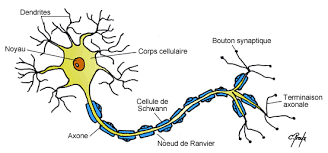
\includegraphics[scale=1]{neurone.png}
\caption{Schéma d’un neurone biologique}
\end{figure}
\subsubsection{Définition}
L'idée de neurone artificiel n’a pas encore été vraiment spécifiée. Au sein d'un processeur, l’unité logique se compose de transistors ; on pourrait également y trouver un réseau neuronal « câblé », mais il faudrait qu’il soit « adaptatif », qu’il ait une « capacité d'apprentissage ». En effet, la réponse d'un neurone à des impulsions entrantes doit pouvoir évoluer tout au long du processus d'apprentissage. C'est ce qu'on appelle la « pondération » : un neurone évalue (pondère) diverses variables d'entrée pour obtenir la variable de sortie souhaitée. C'est pourquoi les neurones sont généralement des fonctions mathématiques qui relient entre elles des variables d'entrée et de sortie [10].

Dans la phase d'apprentissage, les neurones modifient leur comportement de pondération et affinent les résultats de sortie en fonction des variables d'entrée. Il doit donc y avoir un retour d'information du résultat global qui influence chaque neurone. On peut donc dire que les variables d'entrée et de sortie d'un réseau neuronal sont connues, mais que les valeurs des neurones, surtout dans les couches cachées restent inconnues. On a affaire à une « boîte noire » [10].

Pris isolément, un réseau neuronal qui n’a pas été entraîné ne « connaît » rien et fournit des résultats aléatoires, voire chaotiques pour l’utilisateur. Seul un système entraîné fournira le résultat souhaité. Si le problème posé est simple, un programme simple, plus facile à déboguer, pourra le résoudre. Pour un problème plus complexe, on aura recours à un réseau de neurones, que l’on entraînera à l’aide de grands ensembles de données. Chaque neurone peut fournir des variables de sortie complexes et réagir linéairement ou non linéairement aux variables d'entrée.

C'est là un point assez subtil, car les neurones doivent être en mesure de réagir à l’ensemble des possibilités afin de fournir un résultat adéquat. Ceci implique deux choses: soit le programmateur du réseau neuronal connaît toutes les connexions possibles internes au réseau, soit il conçoit le réseau de manière si complexe qu'il couvre « toutes » les possibilités [10].
\begin{figure}[h]
\centering
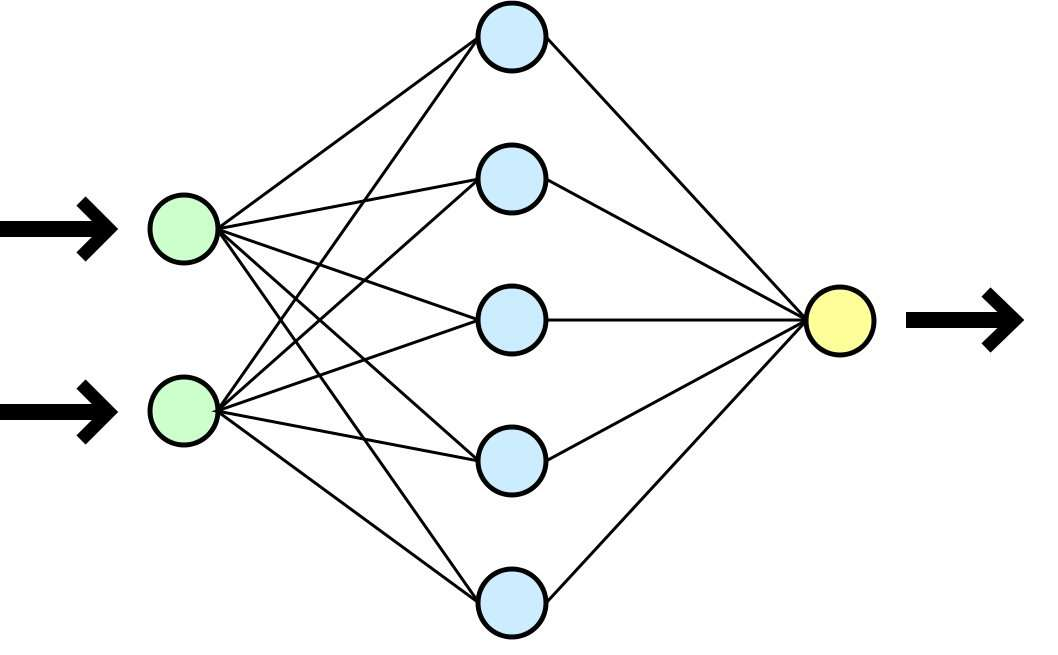
\includegraphics[ height=10cm, width=13cm]{shemadenourone.jpg}
\caption{Schéma d’un réseau artificiel de neurones}
\end{figure}
\newpage
\section{Traitement d’Image (Image Processing)}
\subsection{Introduction}
Les images sont le moyen le plus courant et le plus pratique de transmettre ou de transmettre des informations. Une image vaut mieux que mille mots. Les images transmettent de manière concise des informations sur les positions, les tailles et les relations entre les objets. Ils décrivent des informations spatiales que nous pouvons reconnaître en tant qu'objets. Les êtres humains sont capables de tirer des informations de telles images, grâce à nos capacités mentales et visuelles innées. Environ 75\% des informations reçues par l'homme sont sous forme graphique.

\subsection{L’image numérique}
Une image numérique est la représentation d'une image en deux dimensions avec un ensemble de nombres déterminés d'ensembles finis de valeurs numériques appelées éléments d'image ou pixels. Les valeurs de pixels représentent généralement les niveaux de gris, les couleurs, les hauteurs, les opacités, etc. Chaque pixel est un nombre représenté par un nombre numérique qui représente le degré de confiance d'une zone relativement petite dans une scène. La plage de valeurs nombre numérique étant normalement comprise entre 0 et 255. La taille de cette zone affecte la reproduction des détails dans la scène. Au fur et à mesure que la taille du pixel est réduite, plus de détails de la scène sont préservés en représentation numérique [12].

Une image numérique $a[m, n]$ décrite dans un espace discret 2D est dérivée d'une image analogique a $(x, y)$ située dans un espace continu 2D par le biais d'un processus d'échantillonnage appelé fréquemment numérisation. L'effet de la numérisation est illustré à la figure 3. L'image continue 2D a $(x, y)$ est divisée en N lignes et M colonnes. L'intersection d'une ligne et d'une colonne est appelée un pixel. La valeur attribuée aux coordonnées entières [m, n] avec \{m = 0,1,2, ..., M - 1\} et \{n = 0,1,2, ..., N - 1\} est un $[m, n]$. En fait, dans la plupart des cas, un $(x, y)$ - que nous pourrions considérer comme le signal physique qui frappe la face d’un capteur 2D - est en fait une fonction de nombreuses variables, notamment la profondeur $(z)$, la couleur $(\Lambda)$ ,  et le temps (t) [13].
\newpage
\begin{figure}[h]
\centering
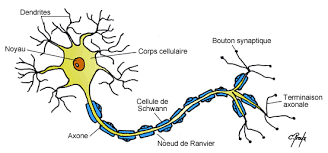
\includegraphics[scale=1]{neurone.png}
\caption{Schéma d’un neurone biologique}
\end{figure}

L'image présentée à la figure 3 a été divisée en N = 16 lignes et M = 16 colonnes. La valeur attribuée à chaque pixel est la luminosité moyenne dans le pixel arrondis à la valeur entière. Le processus de représentation de l'amplitude du signal 2D à une coordonnée donnée sous forme de valeur entière avec L niveaux de gris différents est généralement appelé quantification d'amplitude ou simplement quantification.
\subsection{L’image thermique}
L'image thermique représente la répartition structurée des données représentatives du rayonnement infrarouge en provenance d'une scène thermique (Norme AFNOR A 09-400).

Tout corps dont la température est supérieure au zéro absolu émet en permanence un rayonnement électromagnétique. Le rayonnement thermique est le phénomène d'écoulement de la chaleur par lequel l'énergie calorique se transmet entre deux objets de température différente et séparés dans l'espace par un milieu transparent. Le spectre des radiations électromagnétiques est divisé arbitrairement en un certain nombre de régions déterminées en fonction des générateurs ou récepteurs appropriés (C. Sirieix, 1990a).

Le spectre infrarouge est divisé en trois grandes régions suivant les capteurs utilisables pour les déceler (Gaussorgues, 1989):
\begin{enumerate}
	\item de 0,75 à 1,5 um, l'infrarouge proche décelé par les émulsions photographiques
	\item de 1,5 à 20 um, l'infrarouge moyen décelé par des détecteurs thermiques photoconducteurs ou photovoltaïques.
	\item de 20 à 1000 um, l'infrarouge lointain décelé par les détecteurs thermiques.
\end{enumerate}
\newpage
\subsection{Le traitement d’image}
Le traitement et l'analyse d'images peuvent être définis comme "l'acte d'examiner des images dans le but d'en identifier et d'en juger le sens". L'analyste d'images étudie les données de télédétection et tente, via un processus logique, de détecter, identifier, classer, mesurer et évaluer la signification de données physiques. Le traitement numérique de l'image est un ensemble de techniques permettant de manipuler des images numériques par ordinateur. Les données brutes reçues des capteurs d’imagerie sur les plates-formes satellites contiennent des défauts et des carences[14].

Pour surmonter ces défauts et lacunes afin d'obtenir l'originalité des données, celles-ci doivent subir plusieurs étapes de traitement. Cela varie d'une image à l'autre en fonction du type de format d'image, des conditions initiales de l'image, des informations qui vous intéressent et de la composition de l'image[14].
Le traitement des images comprend essentiellement les trois étapes suivantes:
\begin{enumerate}
	\item Importation de l'image avec un scanner optique ou par photographie numérique.
	\item Analyser et manipuler l'image, ce qui inclut la compression des données, l'amélioration de l'image et la détection de motifs qui ne sont pas visible à l’œil humain comme les photographies satellites.
	\item La sortie est la dernière étape dans laquelle le résultat peut être une image modifiée ou un rapport basé sur une analyse d'image.
\end{enumerate}
\begin{figure}[h]
\centering
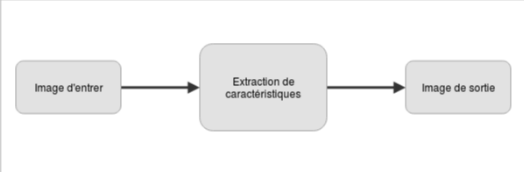
\includegraphics[scale=1, width=13cm]{1.png}
\caption{Présentant les étapes d’un traitement d’une image}
\end{figure}

\subsection{Le but du traitement d'image}
Le traitement de l'image est divisé en 5 groupes. Elles sont:
\begin{enumerate}
	\item Visualisation: Observez les objets non visibles.
	\item Netteté et restauration d'image: Pour créer une meilleure image.
	\item Récupération d'image: Recherchez l'image a la-quel on s’intéresse.
	\item Mesure du motif: Mesure divers objets dans une image.
	\item Reconnaissance d'image: Distinguer les objets dans une image.
\end{enumerate}
\subsection{Les méthodes pour le traitement d’image}
Les deux types de méthodes utilisées pour le traitement d'images sont le traitement d'images analogique et numérique. Des techniques de traitement d'image analogiques ou visuelles peuvent être utilisées pour les copies papier telles que les impressions et les photographies. Les analystes d'images utilisent divers principes d'interprétation lors de l'utilisation de ces techniques visuelles. Le traitement de l'image ne se limite pas à un domaine à étudier, mais à la connaissance de l'analyste. L'association est un autre outil important dans le traitement des images par le biais de techniques visuelles. Les analystes appliquent donc une combinaison de connaissances personnelles et de données collatérales au traitement des images.

Les techniques de traitement numérique aident à manipuler les images numériques en utilisant des ordinateurs. Les données brutes des capteurs d'imagerie contiennent des lacunes et pour surmonter ces défauts et obtenir l’originalité de l’information, l’image doit subir différentes phases de traitement.

Les trois phases générales que doivent subir tous les types de données lors de l’utilisation de la technique numérique sont les suivantes: Prétraitement, Amélioration et Affichage, Extraction d’informations.

\subsection{Les applications existantes}
\begin{enumerate}
	\item Systèmes de transport intelligents - Cette technique peut être utilisée pour la reconnaissance automatique de plaques d'immatriculation et la reconnaissance de panneaux de signalisation [15].
	\item Télédétection - Pour cette application, les capteurs capturent les images de la surface de la Terre dans des satellites de télédétection ou un scanner multispectral monté sur un avion. Ces images sont traitées en les transmettant à la station terrienne. Les techniques utilisées pour interpréter les objets et les régions sont utilisées dans la lutte contre les inondations, la planification urbaine, la mobilisation de ressources, le suivi de la production agricole, etc [16].
	\item Suivi d'objet en mouvement - Cette application permet de mesurer les paramètres de mouvement et d'acquérir un enregistrement visuel de l'objet en mouvement. Les différents types d’approche permettant de suivre un objet sont les suivants: Suivi basé sur le mouvement et suivi basé sur la reconnaissance [17].
	\item Surveillance de la défense - Des méthodes de surveillance aérienne sont utilisées pour surveiller en permanence les terres et les océans. Cette application est également utilisée pour localiser les types et la formation des navires de la surface de l'océan. L'important est de diviser les différents objets présents dans la partie de l'image contenant de l'eau. Les différents paramètres tels que longueur, largeur, surface, périmètre et compacité sont configurés pour classifier chacun des objets divisés. Il est important de reconnaître la répartition de ces objets dans différentes directions (est, ouest, nord, sud, nord-est, nord-ouest, sud-ouest et sud-ouest) pour expliquer toutes les formations possibles des navires. On peut interpréter l'ensemble du scénario océanique à partir de la distribution spatiale de ces objets [18].
	\item Système d'inspection visuelle automatique - Cette application améliore la qualité et la productivité du produit dans les industries.Système d’inspection automatique des filaments des lampes à incandescence - Cela implique un examen du processus de fabrication de l'ampoule. En raison de l’absence d’uniformité dans le pas des câbles de la lampe, le filament de l’ampoule se fond rapidement. Dans cette application, une tranche d'image binaire du filament est créée à partir de laquelle la silhouette du filament est fabriquée. Les silhouettes sont analysées pour reconnaître la non-uniformité du pas du câblage dans la lampe. Ce système est utilisé par la “General Electric Corporation”.
	\begin{enumerate}
		\item Systèmes automatiques d'inspection des surfaces - Dans les industries métallurgiques, il est essentiel de détecter les défauts sur les surfaces. Par exemple, il est essentiel de détecter tout type d'aberration sur la surface du métal laminé dans les laminoirs à chaud ou à froid d'une aciérie. Des techniques de traitement d'image telles que l'identification de texture, la détection de bord, l'analyse fractale, etc. sont utilisées pour la détection.
		\item Identification des composants défectueux - Cette application identifie les composants défectueux dans les systèmes électroniques ou électromécaniques. Une plus grande quantité d'énergie thermique est générée par ces composants défectueux. Les images infrarouges sont produites à partir de la distribution des énergies thermiques dans l'assemblage. Les composants défectueux peuvent être identifiés en analysant les images infrarouges.
	\end{enumerate}
	\item Techniques d'imagerie biomédicale - Pour le diagnostic médical, différents types d'outils d'imagerie tels que les rayons X, les ultrasons, la tomographie assistée par ordinateur (CT), etc. sont utilisés [19]. Certaines des applications des applications d'imagerie biomédicale sont les suivantes:
	\begin{enumerate}
		\item Identification des maladies cardiaques - Il est nécessaire de connaître les caractéristiques de diagnostic importantes telles que la taille du cœur et sa forme afin de classifier les maladies cardiaques. Pour améliorer le diagnostic des maladies cardiaques, des techniques d'analyse d'images sont utilisées pour les images radiographiques [20-21].
		\item Identification des maladies pulmonaires - Dans les rayons X, les régions qui apparaissent sombres contiennent de l'air, tandis que celles qui apparaissent plus claires sont des tissus solides. Les os sont plus radio-opaques que les tissus. Les côtes, le cœur, la colonne thoracique et le diaphragme qui sépare la cavité thoracique de la cavité abdominale sont clairement visibles sur le film radiographique [22-23].
		\item Mammographies numériques - Ceci est utilisé pour détecter la tumeur du sein. Les mammogrammes peuvent être analysés à l'aide de techniques de traitement d'images telles que la segmentation, l'analyse de forme, l'amélioration du contraste, l'extraction de caractéristiques, etc [24].
	\end{enumerate}
\end{enumerate}

\subsection{Les recherches et l’avenir}
Une vaste recherche est en cours dans la technique de traitement d'image.
\begin{enumerate}
	\item Imagerie du cancer - Différents outils, tels que la ponction trachéo-œsophagienne (TEP), l'IRM (Imagerie par Résonances Magnétique) et la détection assistée par ordinateur, aident à diagnostiquer la tumeur et à en prendre conscience.
	\item Imagerie cérébrale - Se concentre sur le développement normal et anormal du cerveau, le vieillissement cérébral et les états pathologiques courants.
	\item Cette recherche intègre l'IRM structurelle et fonctionnelle en neurologie, l'analyse de la forme et de la structure des os, le développement d'outils d'imagerie fonctionnelle en oncologie et le développement de logiciels de traitement d'images TEP [25].
	\item Le développement de la technologie de l'image impose de déterminer si les nouvelles technologies sont efficaces et rentables, et si cette technologie fonctionne dans les domaines tel-que:
	\begin{enumerate}
		\item Imagerie par résonance magnétique du genou.
		\item Détection assistée par ordinateur en mammographie.
		\item Échographie endoscopique dans la stadification du cancer de l'œsophage.
		\item Imagerie par résonance magnétique dans les douleurs lombaires.
		\item Imagerie ophtalmique - Cela fonctionne dans deux catégories:
		\begin{enumerate}
			\item Technologie d'imagerie - Technologie d'imagerie - Développement d'un logiciel automatisé - Analyse les images de la rétine pour montrer les signes précoces de rétinopathie diabétique
			\item Développement de l'instrumentation - Se concentre sur le développement de l'ophtalmoscope à balayage laser.
		\end{enumerate}
	\end{enumerate}
\end{enumerate}

\subsection{Conclusion}
Nous sommes tous en pleine révolution déclenchés par le développement rapide de la technologie informatique et de l'imagerie. Contrairement aux idées reçues, les ordinateurs ne sont pas en mesure d’associer les humains aux calculs liés au traitement et à l’analyse des images.

Mais avec la sophistication croissante et la puissance de l'informatique moderne, le calcul ira au-delà de l'architecture séquentielle conventionnelle de “Von Neumann” et envisagera également l'exécution optique. Les paradigmes de l'informatique distribuée et parallèle devraient améliorer les réponses pour les résultats du traitement des images.
\newpage
\bibliographystyle{ieeetr}	
\bibliography{References}
	

\end{document}
